% Journal Club Talk Poster v5
% for Radio Cosmology Research laboratory, Universiti Malaya
% Designed by Affan Adly Nazri

\documentclass[a4paper]{article}

\usepackage{fontspec}
\setmainfont{MerriweatherSans}[
    Path=./fonts/,
    Scale=1.0,
    Extension=.ttf,
    BoldFont=*-Bold,
    ItalicFont=*-Italic,
    BoldItalicFont=*-BoldItalic,
]
\setmonofont{FiraMono}[
    Path=./fonts/,
    Scale=1.0,
    Extension=.ttf,
]

\usepackage{amsmath, amssymb}
\usepackage{microtype}
\usepackage{xcolor}
\usepackage{tikz}
\usetikzlibrary{calc, fadings, fit, matrix, shadings}
\usepackage{graphicx}
\usepackage{qrcode}
\usepackage{hyperref}
\usepackage[style=apa6]{biblatex}
\usepackage{etoolbox}

% settings
\input{input}
\newcommand{\BillingText}{Radio Cosmology Research Laboratory presents}
\newcommand{\EventName}{Journal Club}
\newcommand{\Location}{Radio Cosmology Research Laboratory\\Centre of Astronomy and Astrophysics Research\\Department of Physics, Faculty of Science\\Universiti Malaya, Kuala Lumpur, Malaysia}
\newcommand{\MeetingLink}{https://us02web.zoom.us/j/83687159462}
\newcommand{\MeetingID}{836 8715 9462}
\newcommand{\MeetingPW}{888666}
\newcommand{\TimeZone}{GMT+8}
\newcommand{\Contact}{Prof. Zamri Zainal Abidin}
\newcommand{\Phone}{+603 7967 4299}
\newcommand{\Email}{zzaa@um.edu.my}
\definecolor{deepblue}{HTML}{222a5b}
\definecolor{vipurple}{HTML}{440148}
\definecolor{textcolour}{HTML}{ffffff}
\definecolor{highlightcolour}{HTML}{fbba15}
\definecolor{qrcolour}{HTML}{101010}
\newlength{\maxwidth}
\setlength{\maxwidth}{0.8\paperwidth}
\newlength{\maxheight}
\setlength{\maxheight}{0.9\paperheight}
\newlength{\whitespace}
\setlength{\whitespace}{0.02\paperwidth}
\newlength{\profilesize}
\setlength{\profilesize}{0.165\paperwidth}
\newlength{\qrsize}
\setlength{\qrsize}{0.175\paperwidth}
\addbibresource{ref.bib}

% preambles
\newcommand{\highlight}[1]{\textcolor{highlightcolour}{#1}}
\DeclareFieldFormat*{title}{\highlight{#1\addperiod}}
\DeclareFieldFormat{doi}{%
  \iffieldundef{url}
    {doi\addcolon\url{https://doi.org/#1}}
    {doi\addcolon\href{\thefield{url}}{#1}}
}
\ifundef{\Title}{
    \ifundef{\CiteKey}{
        \newcommand{\Title}{\fullcite{main}}
    }{
        \newcommand{\Title}{\fullcite{\CiteKey}}
    }
    \newcommand{\TitleFont}{\LARGE\bfseries}
}{
    \newcommand{\TitleFont}{\Huge\bfseries}
}

\begin{document}
    \pagenumbering{gobble}
    \boldmath
    \begin{tikzpicture}[remember picture, overlay, shift={(current page.center)}]
        % background and bounds
        \shade[left color=deepblue, right color=vipurple] (current page.south west) rectangle (current page.north east);
        \node[scope fading=west, anchor=center, rotate=270] at (current page.east) {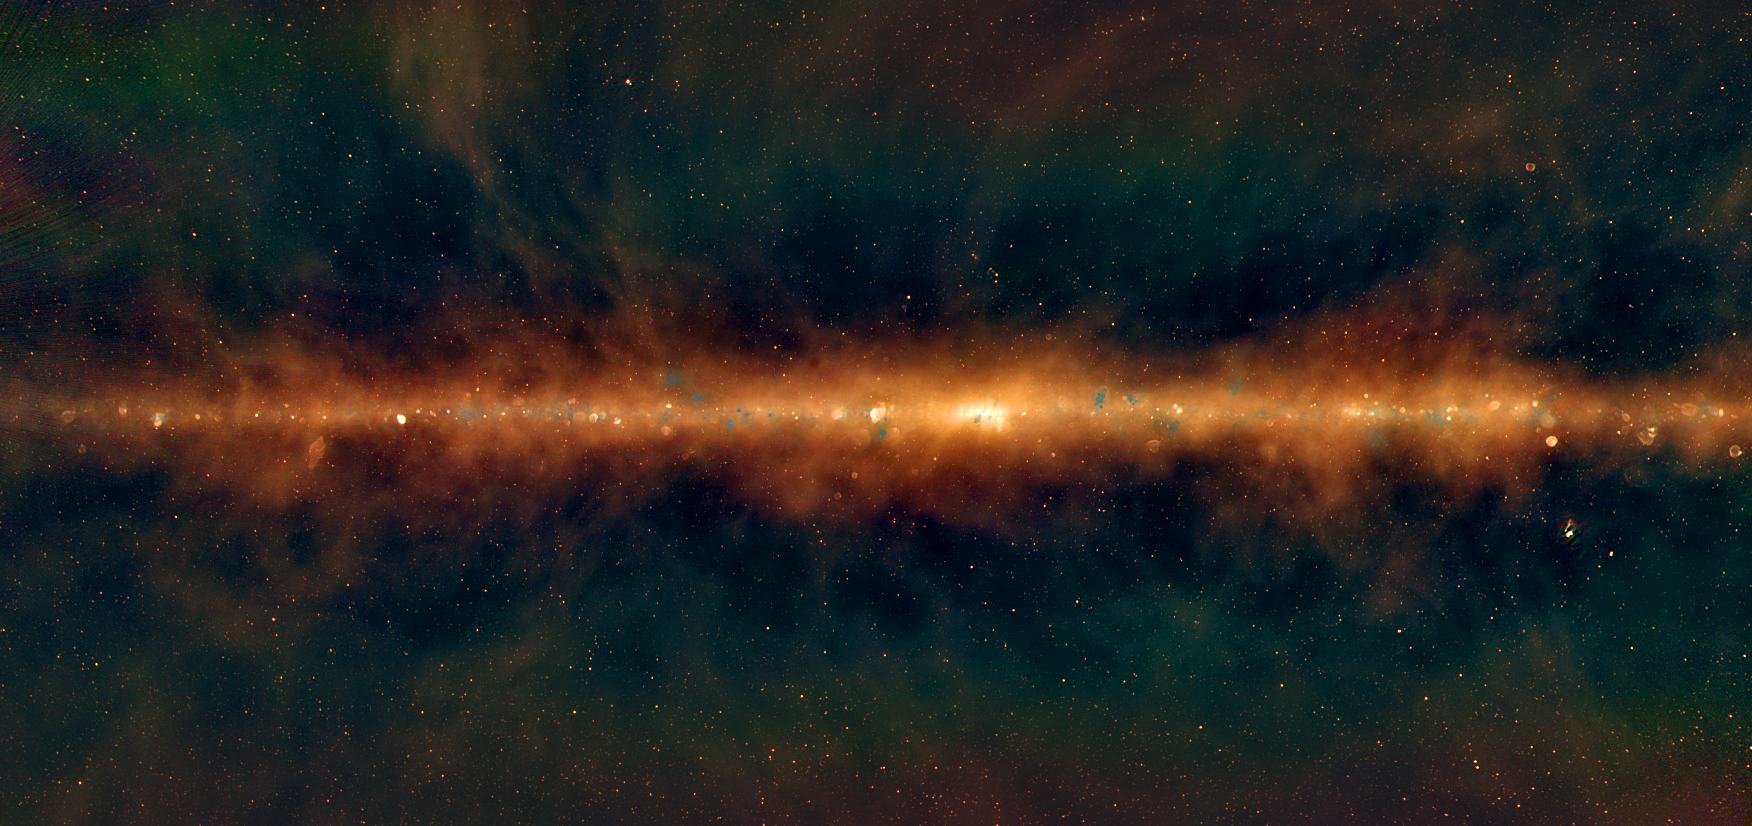
\includegraphics[width=1.2\paperheight]{media/mw_radio.jpg}};
        \node[scope fading=east, anchor=center, rotate=90] at (current page.west) {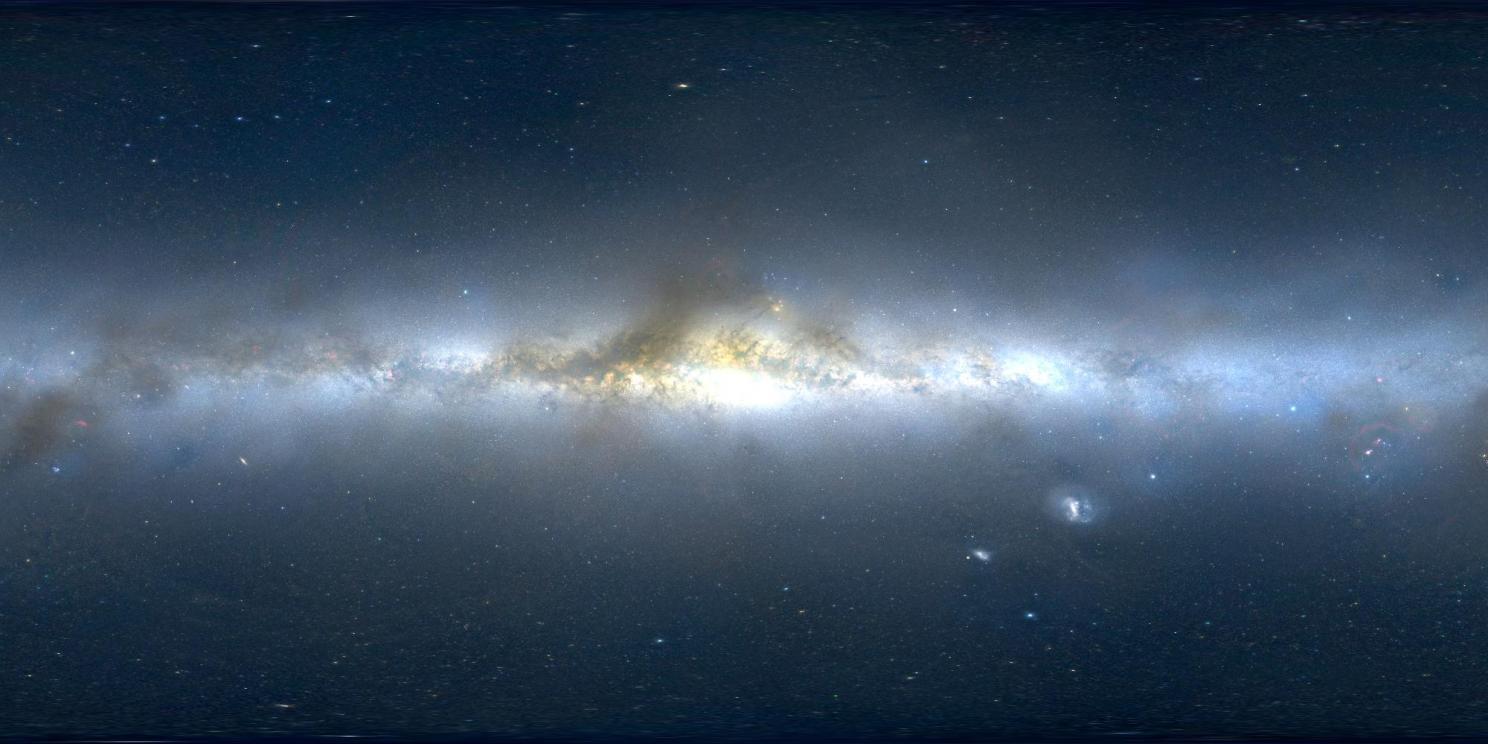
\includegraphics[width=1.2\paperheight]{media/mw_optical.jpg}};
        \coordinate (topleft) at ($(current page.north west)+(0.5*\paperwidth-0.5*\maxwidth,-0.5*\paperheight+0.5*\maxheight)$);
        \coordinate (bottomleft) at ($(current page.south west)+(0.5*\paperwidth-0.5*\maxwidth,0.5*\paperheight-0.5*\maxheight)$);
        \coordinate (bottomright) at ($(current page.south east)+(-0.5*\paperwidth+0.5*\maxwidth,0.5*\paperheight-0.5*\maxheight)$);

        % header
        \node[anchor=north west] (logo) at (topleft) {
            \href{https://sites.google.com/view/radiocosmologylaboratory/home}{\XeTeXLinkBox{
\includegraphics[height=0.055\paperheight]{media/rcl.pdf}}}
            \hspace{\whitespace}
            \href{https://www.um.edu.my}{\XeTeXLinkBox{
\includegraphics[height=0.055\paperheight]{media/um.png}}}
        };

        % footer
        \node[qrcolour, anchor=south east] (qrcode) at (bottomright) {\qrcode[hyperlink, height=\qrsize]{\MeetingLink}};
        \fill[textcolour] (qrcode.north west) rectangle (qrcode.south east);
        \node[qrcolour, anchor=south east] at (qrcode.south east) {\qrcode[hyperlink, height=\qrsize]{\MeetingLink}};
        \node[highlightcolour, font={\large}, text width=0.25\paperwidth, anchor=north east, align=flush right] at ($(qrcode.north west)+(-\whitespace,0)$) {\textbf{Zoom}\\\href{\MeetingLink}{\MeetingID}\\PW: \MeetingPW};
        \node[textcolour, anchor=south east, font={\large}, text width=0.25\paperwidth, align=flush right] (contact) at ($(qrcode.south west)+(-\whitespace,0)$) {\textbf{Contact}\\\Contact\\\Phone\\\href{mailto:\Email}{\Email}};
        \node[textcolour, anchor=north, font={\tiny}] at (qrcode.south) {Credit: Axel Mellinger \& Natasha Hurley-Walker};

        % main matter
        \coordinate (vertical) at ($(logo.south west)!0.5!(qrcode.north east)$);
        \coordinate (center) at (current page.center |- vertical);
        
        \matrix[at=(center), anchor=center, row sep=\whitespace] (main) {
            % billing text
            \node[textcolour, font={\large}, text width=\maxwidth, align=center] (billing) {\BillingText{} \EventName{}}; \\\ifundef{\Profile}{\\}{}

            % presenter
            \node (presenter) {
                \begin{tikzpicture}[baseline=(current bounding box.center)]
                    \ifundef{\Profile}{
                        \node[highlightcolour, font={\Huge\bfseries}, text width=\maxwidth, align=flush left] (name) {\Presenter};
                        \ifundef{\Invited}{
                            \node[highlightcolour, anchor=north west, font={\LARGE\itshape}, text width=\maxwidth, align=flush left] (role) at ($(name.south west)-(0,0.25\whitespace)$) {\Role};
                        }{
                            \node[highlightcolour, anchor=north west, font={\Large}, text width=\maxwidth, align=flush left] (invited) at ($(name.south west)-(0,0.1\whitespace)$) {(Invited Speaker)};
                            \node[highlightcolour, anchor=north west, font={\LARGE\itshape}, text width=\maxwidth, align=flush left] (role) at ($(invited.south west)-(0,0.1\whitespace)$) {\Role};
                        };
                    }{
                       \node[highlightcolour, font={\Huge\bfseries}, text width={\maxwidth-\profilesize-\whitespace}, align=flush left] (name) {\Presenter};
                        \ifundef{\Invited}{
                            \node[highlightcolour, anchor=north west, font={\LARGE\itshape}, text width={\maxwidth-\profilesize-\whitespace}, align=flush left] (role) at ($(name.south west)-(0,0.25\whitespace)$) {\Role};
                            \node[fit=(name)(role), inner sep=0] (presenterblock) {};
                        }{
                            \node[highlightcolour, anchor=north west, font={\Large}, text width={\maxwidth-\profilesize-\whitespace}, align=flush left] (invited) at ($(name.south west)-(0,0.1\whitespace)$) {(Invited Speaker)};
                            \node[highlightcolour, anchor=north west, font={\LARGE\itshape}, text width={\maxwidth-\profilesize-\whitespace}, align=flush left] (role) at ($(invited.south west)-(0,0.1\whitespace)$) {\Role};
                            \node[fit=(name)(invited)(role), inner sep=0] (presenterblock) {};
                        };
                        \node[inner sep=0pt, anchor=west] (profile) 
                            at ($(presenterblock.east)+(\whitespace,0)$) {
                            \begin{tikzpicture}[baseline=(current bounding box.center)]
                                \clip circle (0.5\profilesize);
                                \node[inner sep=0, anchor=center] {\includegraphics[width=\profilesize]{\Profile}};
                            \end{tikzpicture}
                        };
                    }
                \end{tikzpicture}
            }; \\\ifundef{\Profile}{\\}{}
            
            % title
            \node[textcolour, font={\TitleFont}, text width=\maxwidth, align=flush left] (title) {\Title}; \\\\
            
            % time and location
            \node[highlightcolour, font={\LARGE}, text width=\maxwidth, align=flush right] (date) {\Time{} (\TimeZone{}) -- \Date{} (\Day{})}; \\
            \node[textcolour, font={\Large}, text width=\maxwidth, align=flush right] {\Location}; \\
        };
    \end{tikzpicture}
\end{document}